\section{Theoretical backgrounds}
\subsection{Nuclear spin}
Assuming a particles bescribed by its wavefunction $\Psi$, we can describe 
its fundamental properties by quantum numbers corresponding to eigenstates
of different operators. Aside from the quantum number $n$ corresponding to the 
Hamiltonian $\hat{H}$ and thus to the energy level, particles can be further characterized 
by the orbital angular momentum quantum number $l$ and the spin quantum number 
$s$ as well as the projections of both of them onto the $z$-axis, given by 
$m_l$ and $m_s$, respectively. For the nucleus with wavefunction $\Psi_N$, 
spin and angular momentum are coupled to the 
nuclear spin with corresponding operator $\hat{I}$. Its properties are given by:
\begin{align}
    \hat{\mathbf{I}} \Psi_N &= \mathbf{I} \Psi_N \\ 
\intertext{for which}
    \mathbf{I}^2 &= \hbar^2 I(I + 1)
    \label{eq:I_abs}\\
    \left[\hat{H}, \hat{I}^2\right]_- &= 0 
    \label{eq:I_H}\\
\end{align}
While \eqref{eq:I_abs} specifies the absolute value of $\mathbf{I}$, the commutator relation 
\eqref{eq:I_H} ensures that $I$ is constant in time und thus a 'good quantum number'.
For the quantum number of nuclear spin we have $I \in {0, \frac{1}{2}, 1, \ldots}$, while $\hbar$ is the 
reduced Planck constant. A second constant quantum number corresponding to the nuclear spin can be defined:
the projection on the $z$-axis, which in the experiment is given by the direction of the external $B$-field.
It is given by
\begin{align}
    I_z &= m_I \hbar \\
    m_I &\in \left\{-I, -I + 1, \ldots, I - 1, I\right\}
\end{align}
Thus we have $2I + 1$ values for $m_I$, which due to its determining role in the Zeeman effect is 
also called \emph{magnetic quantum number}. Depending on whether $I$ is integer or half integer
we have to apply Bose- or Fermi-statistics; the particles are called bosons or fermions 
accordingly~\cite{Demtroeder1}.

\subsection{Magnetic moment}
Connected to the nuclear spin we observe the \emph{nuclear magnetic moment}
\begin{equation}
    \mu_N = \gamma_N \mathbf{I},
\end{equation}
where $\gamma_N$ is the \emph{gyromagnetic ratio} for the nucleus, which 
can be written in terms of the \emph{nuclear magneton} $\mu_K$
as
\begin{equation}
    \gamma_N = \frac{g_N \mu_K}{\hbar} \, .
\end{equation}
The dimensionless \emph{nuclear g-factor} $g_N$ depends on the constituents of the 
nucleus and is a quantity experimentally measured. $\mu_K$ is defined 
analogously to the Bohr magneton $\mu_B$, but for protons, such that 
\begin{equation}
    \mu_K := \frac{\hbar e}{2 m_p} \, .
\end{equation}
with elementary charge $e = 1.602\mathrm{e}-19$ A s 
and proton mass $m_p = 1.673\mathrm{e}-27$~kg~\cite{Demtroeder1}.
As ferminons, protons and neutrons follow the Pauli principle of exclusion. 
Having spin $S_N = \frac{1}{2}$, there are two possible 'orientations' for 
the $z$-component, namely $m_{s_N} = \pm \frac{1}{2}$. Thus, one orbital 
is filled with two particles of opposite spin. A nucleus can then be 
characterized by the number of protons and neutrons each being 
even ('g') or odd ('u'). A 'gg' nucleus thus has total nuclear spin $I = 0$, 
as for example the case for ($_8^{16}$O)- and ($_6^{12}$C)-atoms. 
'gu' and 'ug' nuclei have $I = \frac{1}{2}$, like the 'ug' ($^1$H) isotope 
measured in this experiment as the only non-zero spin component both of 
glycol (C$_2$H$_6$O$_2$) and water (H$_2$O). The other probe under consideration, 
the $_9^{19}$F with 9 protons and 10 neutrons, 
also has a 'ug' nucleus and thus $I = \frac{1}{2}$, but a different nuclear g-factor. 
Nuclei with odd numbers of 
protons and neutrons have spin $I = 1$; they are aligned parallel due to a lower 
energy stemming from the quark structure of the nucleons respect to the anti-parallel 
alignment with zero nuclear spin. An example is the deuterium $^2$H. However, in this 
experiment we will not look at this case. 

\subsection{Nuclear magnetic resonance}
The energy of a magnetic dipole $\mu$ in an external field $\B$ is given by 
\begin{equation}
    E = - \mu_N \cdot \B
\end{equation}
in both the classical and the quantum mechanical case. In the latter, 
we take the projection of $\mu$ onto the direction of $\B$ with magnitude 
$B := |\B|$ and thus obtain 
\begin{equation}
    E = - g_N \mu_K m_I B \, .
\end{equation}
An energy level which prior to switching on the magnetic field is degenerate in $m_I$ 
will thus be subject to the \emph{Zeeman effect}, describing the split up into two 
distinct levels with difference in energy $\Delta E$. Since $\Delta m_I = 1$, the 
distance between the two levels is given by 
\begin{equation}
    \Delta E = - g_N \mu_K B \, .
\end{equation}
In order to 'flip spins', i.~e. to change state from $m_I = - \frac{1}{2}$ to $m_I = + \frac{1}{2}$, 
or vice versa, the energy has to be absorped or released. The source for absorption can be a photon $\gamma$
of the corresponding energy, thus with frequency 
\begin{equation}
    \Delta \nu = \frac{\Delta E}{h} = \frac{g_N \mu_K B}{h} = \frac{\gamma_N B}{2 \pi}\, .
\end{equation}
The frequency band is widened by the typical effects, such as natural width, Doppler effect 
and collisions. 
In order to examine the effect of a probe on the energy of an external field, there are several
aspects to look at. At first glance, one might come to the conclusion, that the effects of 
absorping photons of the field and those photons being added to the field cancel each other. 
This is not the case though, because of the following reasons:
\begin{itemize}
    \item
        The spontaneous emission is distributed isotropically, such that these photons are lost for 
        the external field along one axis.
    \item
        The number of atoms in the two states is not equal, since the states are distributed according to 
        a Boltzmann distribution, namely $n_{m_I} \propto \exp\left\{-\frac{E_{m_I}}{kT}\right\}$. 
        Thus we can write the ratio of the two occupation numbers by
        \begin{equation}
            \frac{n_{+1/2}}{n_{-1/2}} 
                = \exp\left\{-\frac{E_{+1/2} - E_{-1/2}}{kT} \right\}
                = \exp\left\{-\frac{\Delta E}{kT} \right\} \, .
        \end{equation}
        We conclude that the number of states with $m_I = -\frac{1}{2}$ is higher than the energetically 
        higher state with $m_I = +\frac{1}{2}$. Thus, more photons are absorped than emitted. 
\end{itemize}
One would now expect this latter effect to cease after some time, as $n_{+1/2}$ raises at the expense of 
$n_{-1/2}$. However, there are relaxation processes that keep up the imbalance between the two. 
Apart from spontaneous emission, there is the spin-lattice relaxation allows $\Delta E$ to be passed 
over to the lattice without radiation, such that the energy is lost to the field. 
Yet another effect is the spin-spin interaction which changes the external $\B$-field of atoms close 
to a flipped spin slightly with respect to the case without flip. This results in widening of the 
absorption line. 

\subsection{Hall effect and sensor}
If we look at a conductor with an applied current, which located inside of an magnetic field
(see figure~\ref{fig:halleffect}), the Lorentz force
\begin{equation}
    F = q ( E + v \times B)
\end{equation}
acts on the moving charges such that perpendicular to the direction of the current we will have a potential,
which compensates the Lorentz force:
\begin{equation}
    e E_H = -e v \times B
\end{equation}
By integrating over the distance $b$ of the conducter and supposing a linear
relationship, we arrive at:
\begin{equation}
    U_H = - b v B
\end{equation}
which can be expressed in terms of the Current $I = d \cdot c \cdot j$ where $d$ is the width of the 
conducter and $j=e n v$ the current density:
\begin{equation}
    U_H = \frac{- I\cdot B}{e\cdot n\cdot d}  = -A_H \frac{I\cdot B}{d}
\end{equation}
where we introduced the Hall-coefficient $A_H =\frac{1}{e\cdot n}$ of the material.
\begin{figure}[htpb]
    \centering
    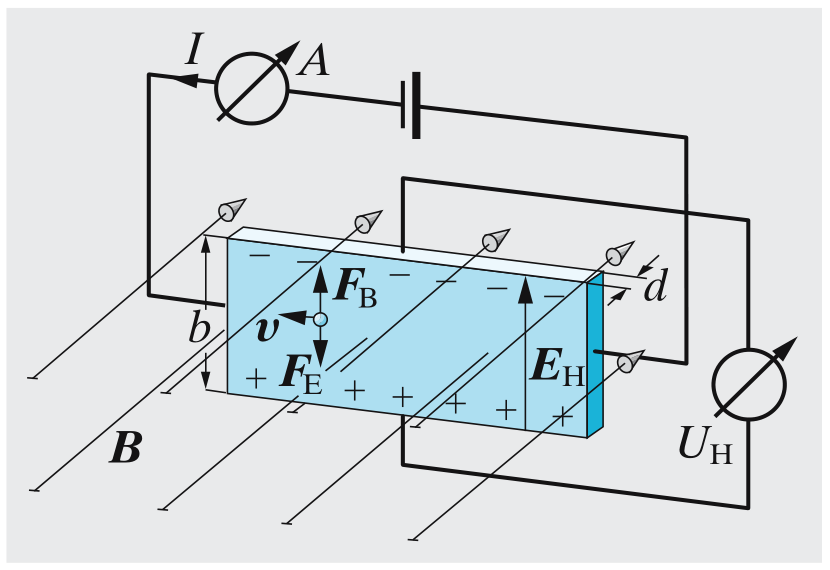
\includegraphics[width=0.8\linewidth]{figures/halleffect}
    \caption{This is the conducter we are talking about in the introduction \cite{gerthsen} to the hall effect.
    The lorentz force is driving the charges perpendicular to the magnetic field until the potential is 
    high enough for the charges to saturate.}
    \label{fig:halleffect}
\end{figure}





\subsection{Lock-in method}
\subsubsection{General Idea}
\label{ssub:General Idea}

In order to supress noise and frequencies from other processes, we use
a frequently used method called ``lock-in amplification''
(see~\cite{lockin} for more details). Depending on your
setup it is possible to reduce the noise by a factor $10^6$. The method
is based on the orthogonality relation of sinusoidal functions (which
can be seen easily if you differentiate the left with respect to $x$):
\begin{equation}
    \int \sin(a x) \sin(b x) dx =\frac{ b \sin(a x) \cos(b x)-a \cos(a x)
            \sin(b x)}{a^2-b^2}
\end{equation}
If we let the integration go from $\infty$ to $-\infty$ we end up with:
\begin{equation}
    (a,b) := \int_{-\infty}^{\infty} \sin(a x) \sin(b x) dx = \delta(a - b)
\end{equation}
Which stems from the sinusoidal functions forming a complete basis with
the integral as inner product.
Since we cannot use the integral over the whole real line, we have to rely
on shorter times: 
\begin{equation}
    (a,b)_t := \int_{0}^{t} \sin(a x) \sin(b x) dx = \delta(a - b)
\end{equation}
\paragraph{case 1: $t = 2k\pi /a$:}
\begin{equation}
    (a,b)_{2\pi /a} = \frac{a \sin(2\pi k\frac{a}{b})}{b^2 - a^2}
\end{equation}
\paragraph{case 1: $t = 2k\pi /b$:}
\begin{equation}
    (a,b)_{2\pi /b} = \frac{b \sin(2\pi k\frac{a}{b})}{a^2 - b^2}
\end{equation}
We notice we can distinguish whether the frequencies are equal or not 
since there is a singularity, but with restrictions~\cite{lockin}:
\begin{itemize}
    \item The integral is evaluated continuosly, which is not possible
        in the real case, so the singularity is replaced by peak, which
        has a finite width.
\item As we do not integrate over the whole real line, we see in the two
    cases that higher harmonics (when working with nonlinear phenomena)
    can appear as well, which should be taken into account.
\item The strength which discriminates the $a=b$ from the $a\neq b$ case
    (the effective bandwidth)
    depends on the Ampitude of the reference signal. 
\end{itemize}

Now we can 
use in such a way that we take the input signal, multiply it by a
reference signal and integrate the result over a given time.
We chose the reference signal with a frequency in the range where we
expect our signal frequency to be: \\\\
\begin{tabular}{l|l}
    \textbf{Phase difference} & \textbf{Recieved Signal} \\
    \hline
    $0^\circ$ & maximal\\
    $180^{\circ}$ & minimal \\
    $90^\circ$ or $270^\circ$ & 0 
\end{tabular}
\vspace{0.5cm}\\\\

\subsection{Materiales used in the experiment}

(PTFE, know by the brand name Teflon), 
